\section{Задание №11}

Построить двумерное пуассоновское поле, отвечающее сложному пуассоновскому процессу:
\begin{enumerate}
        \item Первая интерпретация: система массового обслуживания. При этом первая координата поля --- время поступления заявки в СМО (равномерное распределение), вторая --- время её обслуживания (распределение $\chi^2$ с 10-ю степенями свободы).
        \item Вторая интерпретация: система массового обслуживания с циклической интенсивностью $\lambda(t) = \lambda_0 (1 + \cos(t))$ и единичными скачками. Свести данную задачу моделирования неоднородного пуассоновского процесса при помощи метода Льюиса и Шедлера к моделированию двумерного пуассоновского поля, где первая координата имеет равномерное распределение, а вторая --- распределение Бернулли.
        \item Третья интерпретация: работа страховой компании. Первая координата~--- момент наступления страхового случая (равномерное распределение), вторая координата~--- величина ущерба (распределение Парето). Поступление капитала по времени линейно со скоростью $c > 0$, начальный капитал $W > 0$.
        \item Для каждой системы рассмотреть всевозможные случаи поведения системы в зависимости от значения параметров.
\end{enumerate}


\subsection{Система массового обслуживания}

Пусть $\lambda$ --- интенсивность пуассоновского поля. Время поступления новых заявок генерируются таким образом, что
$$
        \Delta t_i = t_i - t_{i-1}
        \sim
        \mathrm{Exp}(\lambda).
$$

\begin{definition}
        \textit{Распределением $\chi^2$ с $k$ степенями свободы} называется распределение суммы квадратов $k$ независимых стандартных случайных величин.
\end{definition}

Время обслуживания $i$-ой заявки обозначим за $s_i$. Эти времена независимы и генерируются как случайные величины с распределением $\chi^2(10)$. Все заявки обрабатываются последовательно. Таким образом, мы можем найти время окончания обработки $i$-ой заявки $Q_i$ так:
$$
        \begin{cases}
Q_i = t_i + s_i, 
        &
\mbox{если $(i-1)$-ая заявка обработана,}
        \\
Q_i = Q_{i-1} + s_i,
        &
\mbox{иначе.}
        \end{cases}
$$
Или, обобщая, можно написать так:
$$
        Q_i
        =
        t_i
        +
        \max\{0,\,Q_{i-1} - t_i\}
        +
        s_i.
$$

Для каждой заявки, мы будем считать количество заявок, ожидающих обработки, на момент прихода данной заявки. То есть количество $n_i$ таких заявок $j$, что
$$
        j < i
        \quad
        \mbox{и}
        \quad
        Q_j > t_i.
$$

Поскольку среднее время обработки одной заявки равен $10$, а средний интервал между поступлениями заявок равен $\E\,\Delta_i = \nicefrac{1}{\lambda}$, то ожидаем отсутствия очереди при $\lambda < 0,\!1$ и неограниченный рост очереди при $\lambda > 0,\!1$.

\clearpage
\begin{figure}[t]
        \noindent
        \centering
        {
        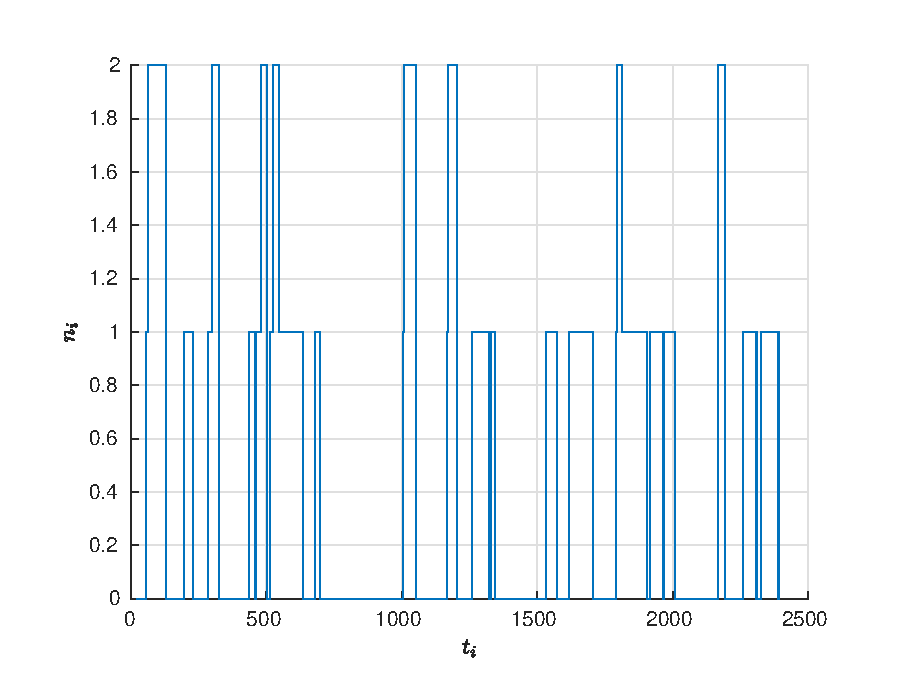
\includegraphics[width=120mm]{task_11/1-l-0-05.eps}}
        \caption{}
\end{figure}
\begin{figure}[b]
\noindent
        \centering
        {
        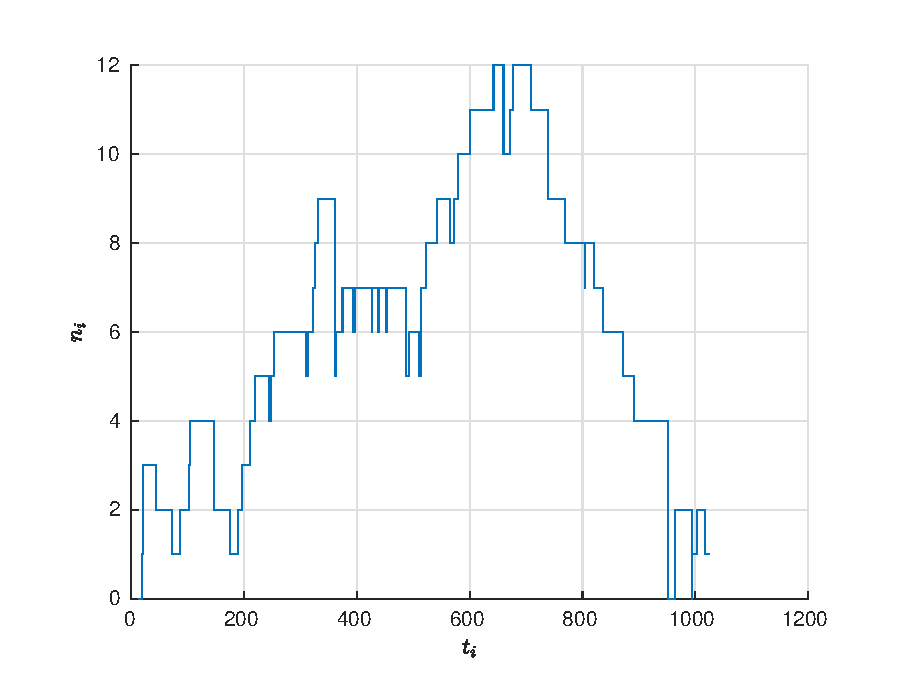
\includegraphics[width=120mm]{task_11/1-l-0-1.eps}}
        \caption{}
\end{figure}
\begin{figure}[h]
\noindent
        \centering
        {
        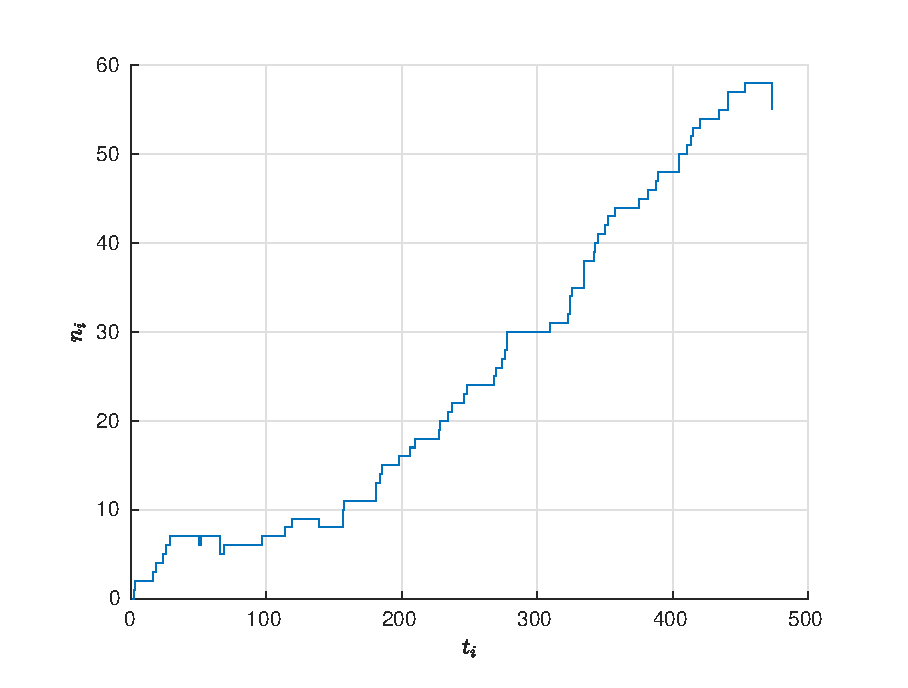
\includegraphics[width=120mm]{task_11/1-l-0-2.eps}}
        \caption{}
\end{figure}


\section{Система массового обслужиания с циклической интенсивностью}

Пусть теперь $t_1,t_2,\ldots,T_n,\ldots$ --- времена наступления некоторых событий, $N(t_1,t_2)$ --- число событий, произошедших в промежуток времени $[t_1,t_2]$. Заметим, что $t_{i+1} - t_i$ имеет функцию распределения
$$
        F(x) = 1 - e^{-(\Lambda(t+x) - \Lambda(t))},
        \quad
        \mbox{где }
        \Lambda(t) = \int\limits_0^t\lambda(u)\,du = \lambda(t + \sin t).
$$
Здесь $x \leqslant 0$, а сам интеграл $\Lambda(t)$ неограничено возрастает при росте $t$.